\chapter{Overview of Finite Element Theory}
\section{Introduction to the method}
\begin{itemize}
	\item Discretisation of the model to elements
	\item Governing equations for each element
	\item Assembled to give system equations
	\item $[k]\{U\} = \{F\}$
	\item $[k]$ is a square matrix, stiffness matrix $\{U\}$ is the vector of unknown nodal displacements or temperatures and $\{F\}$ is the vector of applied nodal forces
\end{itemize}
\section{1D element - the pin jointed bar}
\begin{figure}[H]
	\centering
	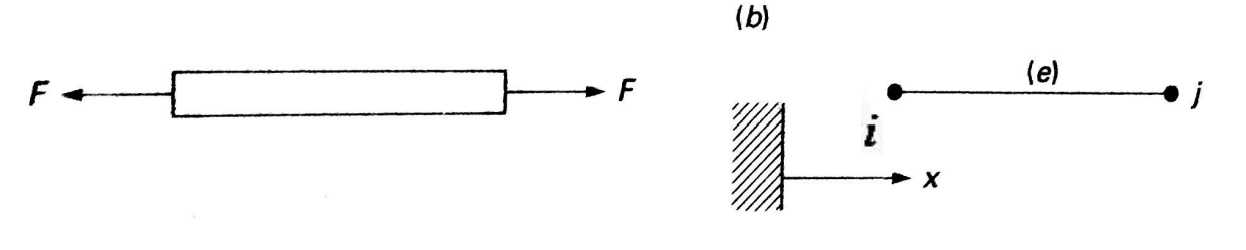
\includegraphics[width = \textwidth]{./img/figure3.png}
	\caption{Pin jointed bar.}
\end{figure}
\begin{align}
	u &= a + bx\\
	u_i &= a + bx_i\\
	u_j &= a + bx_j
\end{align}
where $u_{i,j}$ are unknown nodal displacements and $x_{i,j}$ are known nodal coordinates. This leads to:
\begin{align}
	a &= \frac{\left(u_ix_j-u_jx_i\right)}{L}\\
	b &= \frac{\left(u_j-u_i\right)}{L}\\
	u&= \frac{x_j-x}{L}u_i + \frac{x-x_i}{L}u_j\\
	u &= N_iu_i + N_ju_j
\end{align}
where $L = x_j - x_i$. $N_i$ and $N_j$ are called shape functions. When a structure is loaded and reaches an equilbirium its potential energy must be minimum.
\begin{gather}
	\Pi = \Lambda - W
\end{gather}
where $\Lambda$ is strain energy and $W$ is work done by external loads (pressure load, body force, nodal forces).
\begin{gather}
	W = u_i F_i + u_j F_j = \{U\}^T \{F\}
\end{gather}
where:
\begin{gather}
	\{U\}^T = \begin{bmatrix}
		u_i & u_j
	\end{bmatrix}\\
	\{F\} = \begin{Bmatrix}
		F_i\\
		F_j
	\end{Bmatrix}
\end{gather}
\begin{gather}
	\Lambda = \int_{x_i}^{x_j}\left(\frac{1}{2}\sigma\varepsilon A\right) \dif x
	\Lambda = \frac{AE}{2}\int_{x_i}^{x_j}\left(\varepsilon^2\right)\dif x
\end{gather}
where $\sigma = E\varepsilon$ and is the stress, $\Lambda$ is strain energy density, $A$ is surface area and $x$ is length. Using the definition of strain:
\begin{gather}
	\varepsilon = \frac{\dif u}{\dif x}
\end{gather}
We can differentiate our shape function:
\begin{gather}
	\varepsilon = \frac{\left(-u_i + u_j\right)}{L}
\end{gather}
Leading to:
\begin{gather}
	\Lambda = \frac{AE}{2L}\left(-u_i + u_j\right)^2\\
	\Lambda = \frac{AE}{2L}\begin{bmatrix}
		u_i & u_j
	\end{bmatrix}\begin{bmatrix}
		1 & -1\\
		-1 & 1
	\end{bmatrix}\begin{Bmatrix}
		u_i\\
		u_j
	\end{Bmatrix}\\
	= \frac{1}{2}\{U\}^T[k]\{U\}
\end{gather}
where the stiffness matrix is:
\begin{gather}
	[k] = \frac{AE}{L}\begin{bmatrix}
		1 & -1\\
		-1 & 1
	\end{bmatrix}
\end{gather}
Potential energy must be minimised
\begin{gather}
	\Pi = \frac{1}{2}\{U\}^T [k]\{U\} - \{U\}^T \{F\}\\
	\frac{\partial \Pi}{\partial u_i} = \frac{\partial \Pi}{\partial u_j} = 0 \textrm{ or } \frac{\partial \Pi}{\partial \{U\}} = 0\\
	\frac{\partial \Pi}{\partial \{U\}} = [k]\{U\} - \{F\} = 0\\
	\begin{Bmatrix}
		F_i\\
		F_j
	\end{Bmatrix} = \frac{AE}{L}\begin{bmatrix}
		1 & -1\\
		-1 & 1
	\end{bmatrix}\begin{Bmatrix}
		u_i\\
		u_j
	\end{Bmatrix}\\
	\Pi = \sum^E_{e=1}\left(\Lambda^{\left(e\right)}-W\right)
\end{gather}
Leading to:
\begin{gather}
	\frac{\partial \Pi}{\partial\{U\}} = \left(\sum^E_{e=1}\left[k^{\left(e\right)}\right]\right)\{U\}-\{F\} = 0
\end{gather}
\subsection{Exercise}
Calculate the displacement and stress using the stiffness matrix.
\begin{figure}[H]
	\centering
	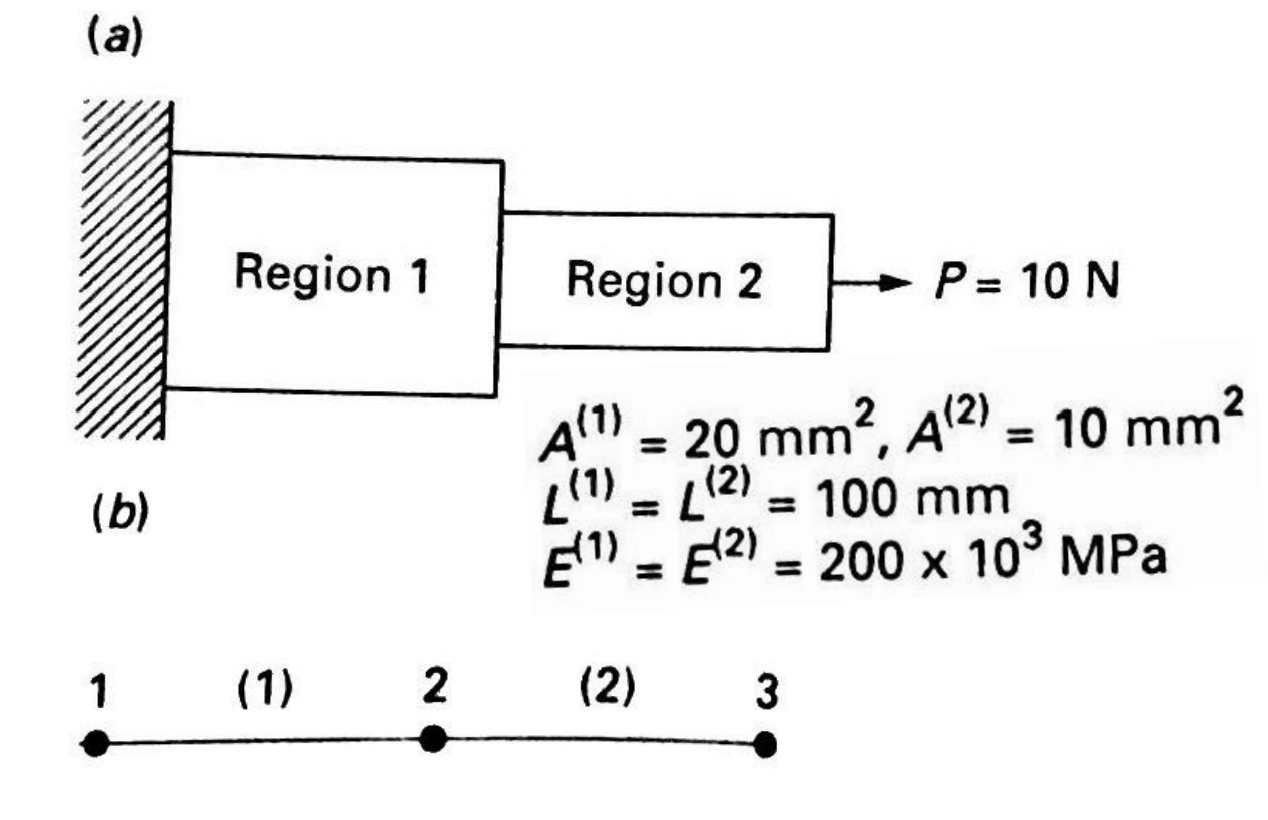
\includegraphics[width = \textwidth]{./img/figure4.png}
	\caption{Exercise, 3 node 1D problem.}
\end{figure}
\begin{gather}
	\left[k_1\right] = \frac{A_1E_1}{L_1} \begin{bmatrix}
		1 & -1\\
		-1 & 1
	\end{bmatrix} = \begin{bmatrix}
		4 & -4\\
		-4 & 4
	\end{bmatrix}\times 10^4\, \si{\newton\per\milli\meter}\\
	\left[k_2\right] = \frac{A_2E_2}{L_2} \begin{bmatrix}
		1 & -1\\
		-1 & 1
	\end{bmatrix} = \begin{bmatrix}
		2 & -2\\
		-2 & 2
	\end{bmatrix}\times 10^4\, \si{\newton\per\milli\meter}\\
	\left[k\right] = \begin{bmatrix}
		4 & -4 & 0\\
		-4 & 6 & -2\\
		0 & -2 & 2\\
	\end{bmatrix}\times 10^4\, \si{\newton\per\milli\meter}\\
	\{F\}^T = \begin{bmatrix}
		0 & 0 & 10
	\end{bmatrix}
	10^4\times\begin{bmatrix}
		4 & -4 & 0\\
		-4 & 6 & -2\\
		0 & -2 & 2\\
	\end{bmatrix}\begin{Bmatrix}
		u_1\\
		u_2\\
		u_3
	\end{Bmatrix} = \begin{Bmatrix}
		0 + R1\\
		0\\
		10
	\end{Bmatrix}
\end{gather}
Leading to (commented in Latex):
\begin{gather}
	u_1 = 0\\
	u_2 = \SI{0.25e-3}{\milli\meter}\\
	u_3 = \SI{0.75e-3}{\milli\meter}\\
	R_1 = \SI{-10}{\newton}\\
	\varepsilon_1 = \frac{\left(-u_1+u_2\right)}{L} = \SI{2.5e-6}{}\\
	\varepsilon_2 = \frac{\left(-u_2+u_3\right)}{L} = \SI{5e-6}{}\\
	\sigma_1 = E\varepsilon_1 = \SI{0.5}{\newton\per\milli\meter}\\
	\sigma_2 = E\varepsilon_2 = \SI{1}{\newton\per\milli\meter}
\end{gather}
\section{1D element - the spring}
Consider the same 1D linear spring with stiffness $k$ independent of deflection:
\begin{figure}[H]
	\centering
	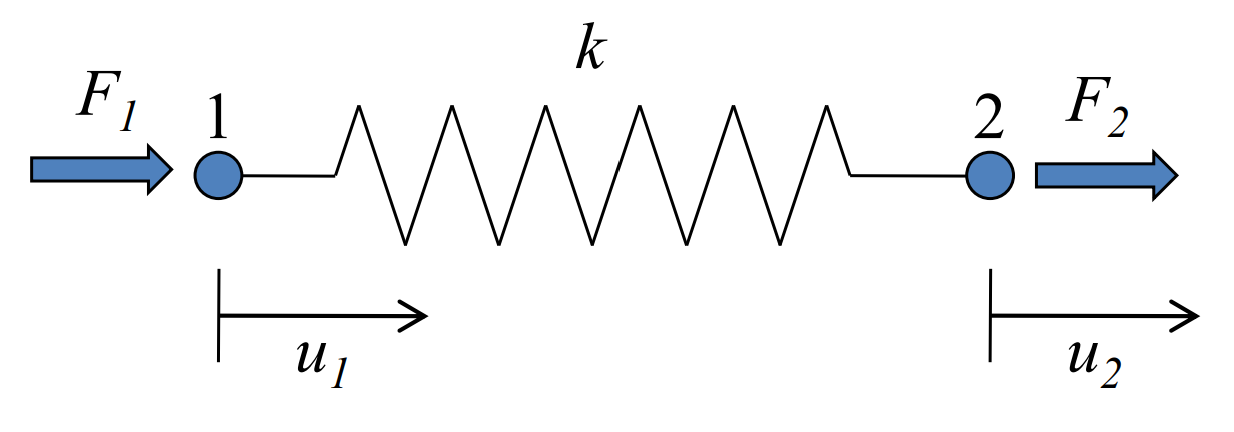
\includegraphics[width = \textwidth]{./img/figure5.png}
	\caption{Spring system.}
\end{figure}
\begin{gather}
	W_{ext} = \int_0^{u_1} \left(F_1(u)\right)\dif u + \int_{0}^{u_2} \left(F_2(u)\right)\dif u\\
	\delta W_{ext} = F_1 \delta u_1 + F_2 \delta u_2 = \begin{pmatrix}
		\delta u_1 & \delta u_2 
	\end{pmatrix} \begin{pmatrix}
		F_1\\
		F_2
	\end{pmatrix}
\end{gather}
where $F_1 = F_1\left(u_1\right)$ and $F_2 = F_2\left(u_2\right)$.
\begin{gather}
	W_{int} = \frac{1}{2}k\left(u_2- u_1\right)^2 = \frac{1}{2}\begin{pmatrix}
		u_1 & u_2
	\end{pmatrix}\begin{bmatrix}
		k & -k\\
		-k & k
	\end{bmatrix}\begin{pmatrix}
		u_1\\
		u_2
	\end{pmatrix}\\
	\delta W_{int} = k\left(u_2 - u_1\right)\left(\delta u_2 -\delta u_1\right) = \begin{pmatrix}
		\delta u_1 & \delta u_2
	\end{pmatrix}\begin{bmatrix}
		k & -k\\
		-k & k\\
	\end{bmatrix}\begin{pmatrix}
		u_1\\
		u_2
	\end{pmatrix}
\end{gather}
Applying the principle of virtual work gives:
\begin{gather}
	\delta W_{ext} = \delta W_{int} \rightarrow \delta u_1 \left[-k\left(u_2 - u_1\right)-F_1\right] + \delta u_2 \left[k\left(u_2 - u_1\right)-F_2\right] = 0
\end{gather}
and since $\delta u_1$ and $\delta u_2$ are arbitrary, one obtains:
\begin{gather}
	F_1 = ku_1 - ku_2 \textrm{ and } F_2 = -ku_1 + ku_2
\end{gather}
Or, in matrix form:
\begin{gather}
	\underline{F} = \begin{pmatrix}
		F_1\\
		F_2
	\end{pmatrix} = \begin{bmatrix}
		k & -k\\
		-k & k
	\end{bmatrix}\begin{pmatrix}
		u_1\\
		u_2
	\end{pmatrix} = \underline{K}\underline{u}
\end{gather}